\documentclass[letterpaper,11pt]{article}
\oddsidemargin -1.0cm \textwidth 17.5cm

\usepackage[utf8]{inputenc}
\usepackage[activeacute,spanish, es-lcroman]{babel}
\decimalpoint
\usepackage{amsfonts,setspace}
\usepackage{amsmath}
\usepackage{amssymb, amsmath, amsthm}
\usepackage{comment}
\usepackage{float}
\usepackage{amssymb}
\usepackage{dsfont}
\usepackage{anysize}
\usepackage{multicol}
\usepackage{enumerate}
\usepackage{graphicx}
\usepackage[left=1.5cm,top=2cm,right=1.5cm, bottom=1.7cm]{geometry}
\setlength\headheight{1.5em} 
\usepackage{fancyhdr}
\usepackage{multicol}
\usepackage{hyperref}
\usepackage{wrapfig}
\usepackage{subcaption}
\usepackage{siunitx}
\usepackage{cancel}
\usepackage{mdwlist}
\usepackage{svg}
\pagestyle{fancy}
\fancyhf{}
\renewcommand{\labelenumi}{\normalsize\bfseries P\arabic{enumi}.}
\renewcommand{\labelenumii}{\normalsize\bfseries (\alph{enumii})}
\renewcommand{\labelenumiii}{\normalsize\bfseries \roman{enumiii})}


\begin{document}

\fancyhead[L]{\itshape{Facultad de Ciencias F\'isicas y Matem\'aticas}}
\fancyhead[R]{\itshape{Universidad de Chile}}
\rfoot[]{pág. \thepage}

\begin{minipage}{11.5cm}
    \begin{flushleft}
        \hspace*{-0.6cm}\textbf{FI1100 Introducción a la Física Moderna}\\
        \hspace*{-0.6cm}\textbf{Tutor:} Alejandro Cartes
    \end{flushleft}
\end{minipage}

\begin{picture}(2,3)
    \put(366, -10){
\includegraphics[scale=0.9]{Imágenes/logo/dfi-fcfm.pdf}}
\end{picture}

\begin{center}
	\LARGE\textbf{Tutoría C1}\\
	\Large{Óptica Geométrica}
\end{center}

\vspace{-1cm}
\begin{enumerate}\setlength{\itemsep}{0.4cm}

\item[]

\section*{\underline{Reflexión y Refracción}}

\rfoot[]{pág. \thepage}

\begin{multicols}{2}
\item El \textit{Principio de Fermat} establece que siempre que la luz viaja desde un punto a otro, su trayectoria real es la que requiere el menor intervalo de tiempo. Considerando la situación de la figura:
    \begin{enumerate}
        \item Demuestre que el tiempo cuando la luz llega a $Q$ es

        $$t = \frac{n_1\sqrt{a^2+x^2}}{c} + \frac{n_2\sqrt{b^2+(d-x)^2}}{c}$$

        \item Para obtener el valor de $x$ para que $t$ alcance su valor mínimo, derive $t$ con respecto a $x$ e iguale la derivada a cero. Demuestre que se tiene la siguiente relación

        \[\frac{n_1x}{\sqrt{a^2+x^2}} = \frac{n_2(d-x)}{\sqrt{b^2+(d-x)^2}}\]

        \item Demuestre que esta expresión corresponde a la ley de Snell
    \end{enumerate}

    \columnbreak

    \begin{figure}[H]
        \centering
        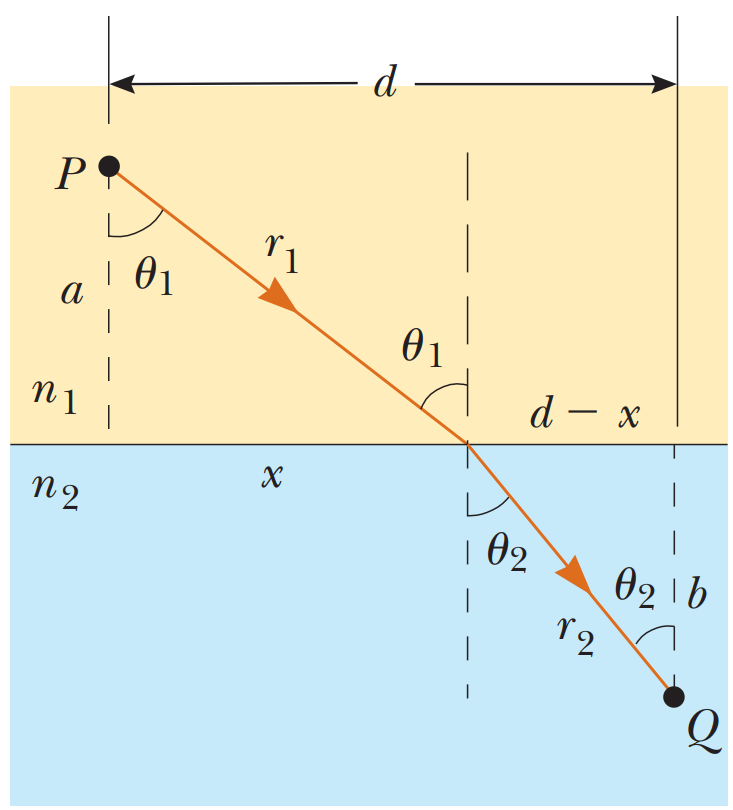
\includegraphics[width=0.8\linewidth]{Imágenes/clases/interfaz.png}
    \end{figure}
\end{multicols}

% \begin{multicols}{2}
%     \item Un material que tiene un índice de refracción $n$ está rodeado por vacío y tiene la forma de un cuarto de círculo de radio $R$. Un rayo de luz paralelo a la base del material incide desde la izquierda a una distancia $L$ por encima de la base y emerge desde el material a un ángulo $\theta$. Determine una expresión para $\theta$
    
%     \columnbreak
    
%     \begin{figure}[H]
%         \centering
%         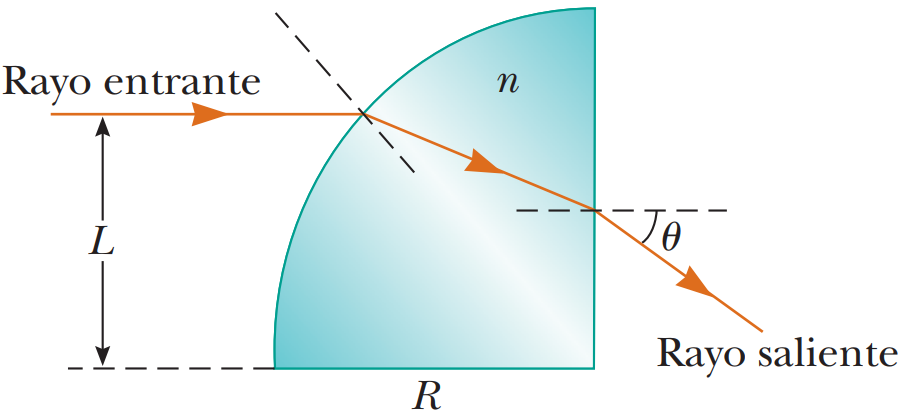
\includegraphics[width=0.75\linewidth]{Imágenes/clases/cuarto-circ.png}
%     \end{figure}
% \end{multicols}

% \begin{multicols}{2}
%     \item Una fibra óptica tiene un índice de refracción $n$ y un diámetro $d$. Se envía un haz de luz por la fibra a lo largo de su eje, como se muestra en la figura. Si la fibra se encuentra rodeada de aire, determine el mínimo radio exterior $R$ permitido para una curva en la fibra si no ha de escapar luz.

%     \columnbreak
    
%     \begin{figure}[H]
%         \centering
%         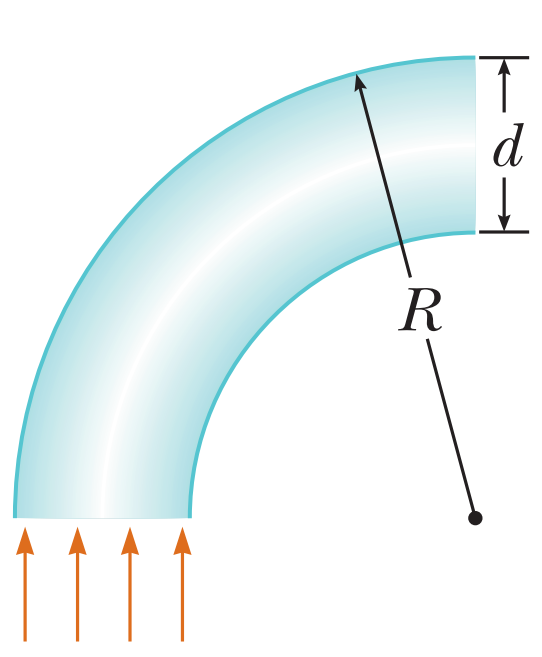
\includegraphics[width=0.3\linewidth]{Imágenes/clases/fibra.png}
%     \end{figure}
% \end{multicols}

\begin{minipage}{0.6\linewidth}
    \item Un pez se encuentra en el fondo de un lago que posee un índice de refracción desconocido. El pez, al alzar la vista en un ángulo $\alpha = 32^{\circ}$ con respecto a la vertical, observa una gaviota. Un cangrejo que iba pasando le menciona al pez que la luz proveniente de la gaviota tiene un ángulo de incidencia $\beta = 49^{\circ}$.
    
    \begin{enumerate}
        \item ¿Cuál es el índice de refracción del agua del lago?
        
        \item El cangrejo advierte que hay otra gaviota cerca y que para verla, el pez tiene que mirar en un ángulo $\gamma = 47^{\circ}$ con respecto a la vertical. ¿Realmente la podrá ver? ¿Por qué?
    \end{enumerate}
\end{minipage}
\hfill
\begin{minipage}{0.35\linewidth}
    \begin{figure}[H]
        \centering
        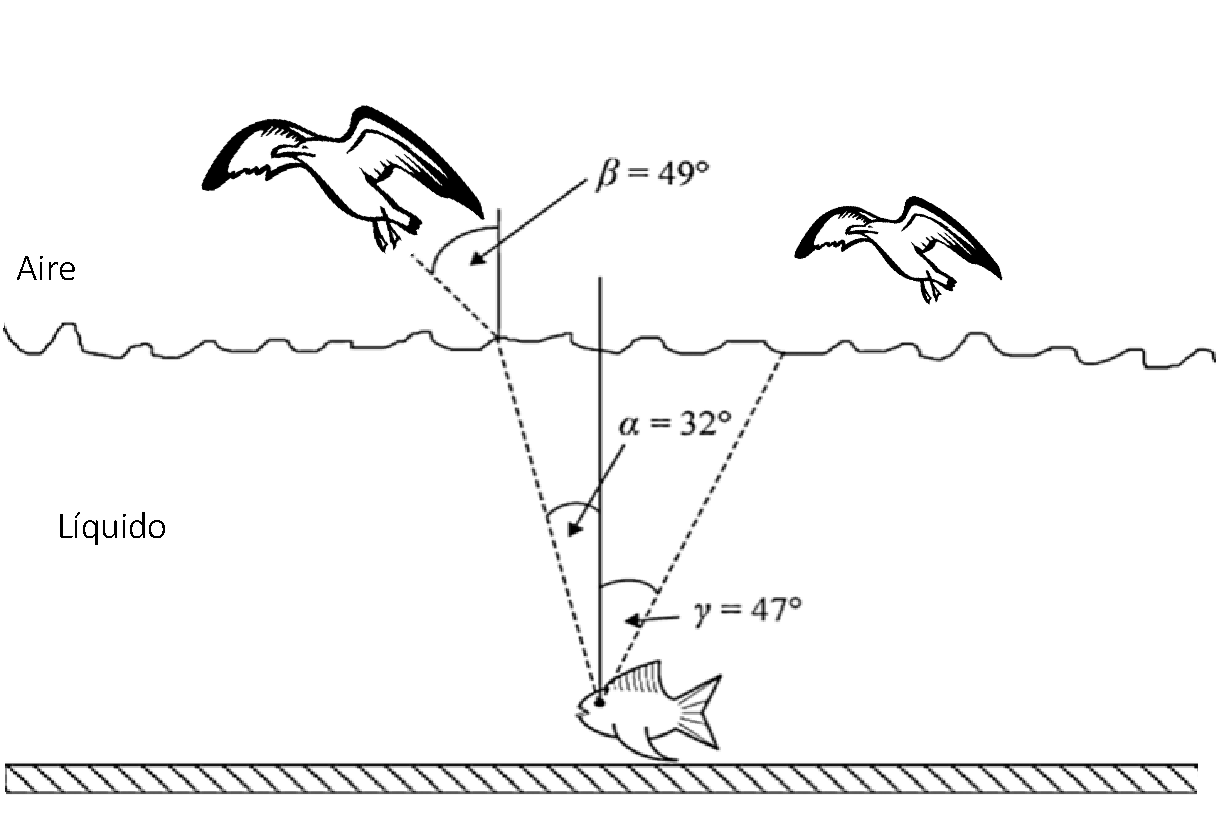
\includegraphics[width=1\linewidth]{Imágenes/aux6/pajaros.pdf}
    \end{figure}
\end{minipage}

\item Un rayo de luz incide sobre la superficie 2 en el ángulo crítico. Determine el ángulo de incidencia $\theta_1$

\begin{figure}[H]
    \centering
    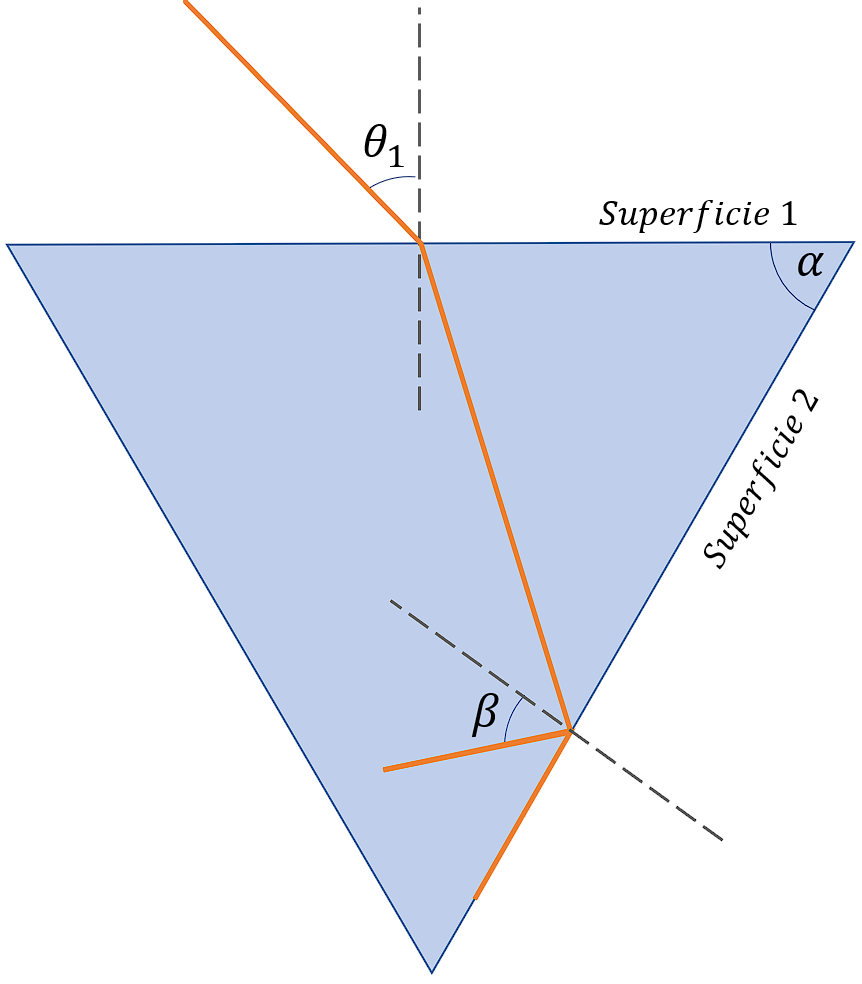
\includegraphics[width=0.23\linewidth]{Imágenes/clases/triangulo.png}
\end{figure}

\end{enumerate}

\section*{\underline{Espejos y Lentes}}
\begin{enumerate}

\item Una persona de altura $h$ desde sus pies hasta sus ojos se para frente a un espejo plano, el cual parte a la altura de los ojos de la persona. ¿Cuál es el largo del espejo para que la persona sea capaz de mirar, a más poder, sus zapatos?

\begin{figure}[H]
    \centering
    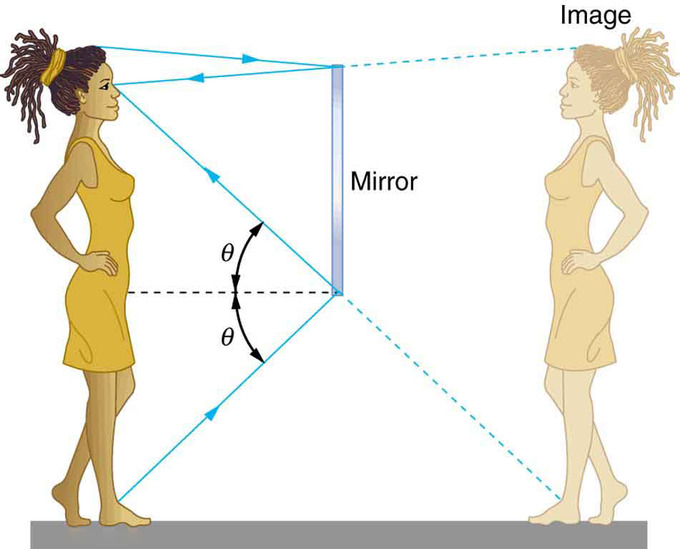
\includegraphics[width=0.2\linewidth]{Imágenes/clases/persona.png}
\end{figure}

\item

\begin{enumerate}
    \item Para un espejo cóncavo de longitud focal $f$, ¿cuál debe ser la distancia $d_0$ del objeto para que la distancia de la imagen sea igual a esta? Dibuje los rayos principales, ¿es una imagen real o virtual?¿derecha verticalmente o invertida?

    \item Cuando un objeto está a cierta distancia de un espejo cóncavo, el aumento de la imagen es $M_1$. Si el objeto se mueve una distancia $\ell$ de su ubicación original, el aumento de la imagen pasa a ser $M_2$. ¿Cuál es la distancia focal de este espejo?
\end{enumerate}

\item Considere un sistema óptico compuesto por una lente convexa con longitud focal $f_L = \SI{0.02}{\m}$ y un espejo convexo $M$ de radio $R_M = \SI{0.12}{\m}$. Si la distancia entre el lente y el espejo es $d=\SI{0.04}{\m}$, determine la ubicación de la imagen de un objeto ubicado a $\SI{0.03}{m}$ de la lente

\begin{figure}[H]
    \centering
    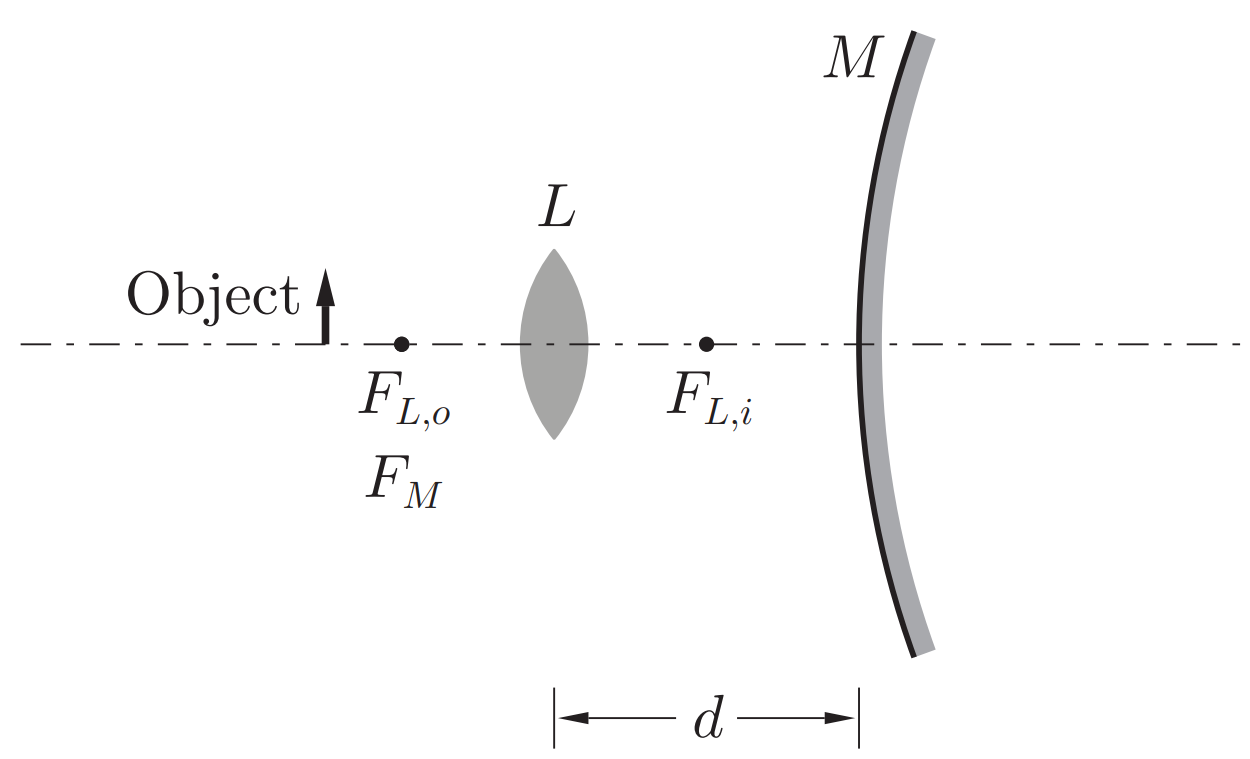
\includegraphics[width=0.3\linewidth]{Imágenes/clases/lens-mirror.png}
\end{figure}

% \item Como se muestra en la figura, tres lentes biconvexos idénticos de distancia focal $f$ son alineados y separados una distancia $f$ entre ellos. Usando rayos principales, encuentre la posición y la magnificación de la imagen resultante si se ubica un objeto a una distancia $f/2$ del lente ubicado más a la izquierda

% \begin{figure}[H]
%     \centering
%     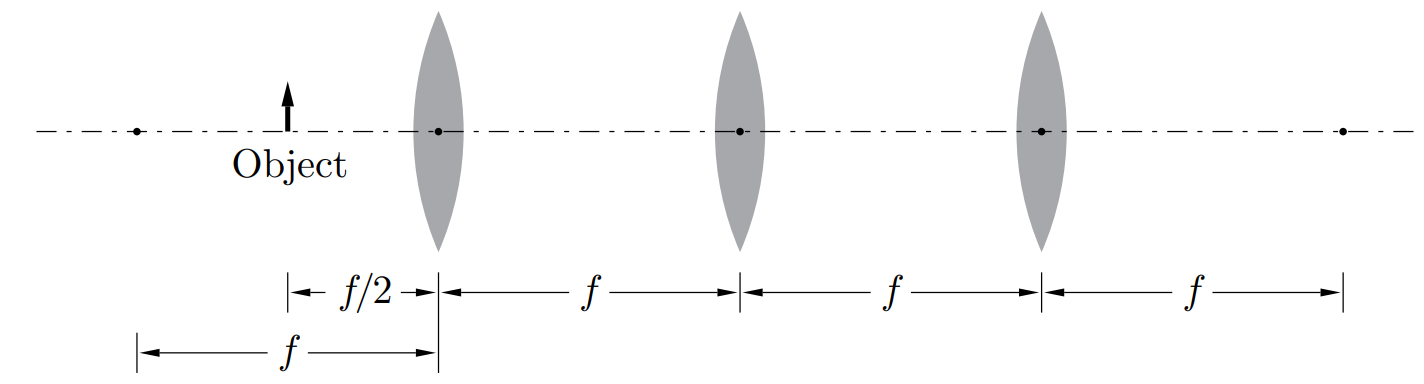
\includegraphics[width=0.35\linewidth]{Imágenes/clases/three-lenses.png}
% \end{figure}

\item Considere el siguiente sistema óptico compuesto por una lente convergente y una divergente. La distancia focal de los lentes son, respectivamente, $f_1=\SI{50}{\mm}$ y $f_2 = \SI{-100}{\mm}$. \textbf{(a)} Determine la distancia $d$ entre el lente divergente y el sensor si el sistema enfoca un objeto que se encuentra a una distancia $\SI{0.5}{\m}$ del lente $L_1$. \textbf{(b)} ¿Cuál es la magnificación de la imagen formada por este sistema?

\begin{figure}[H]
    \centering
    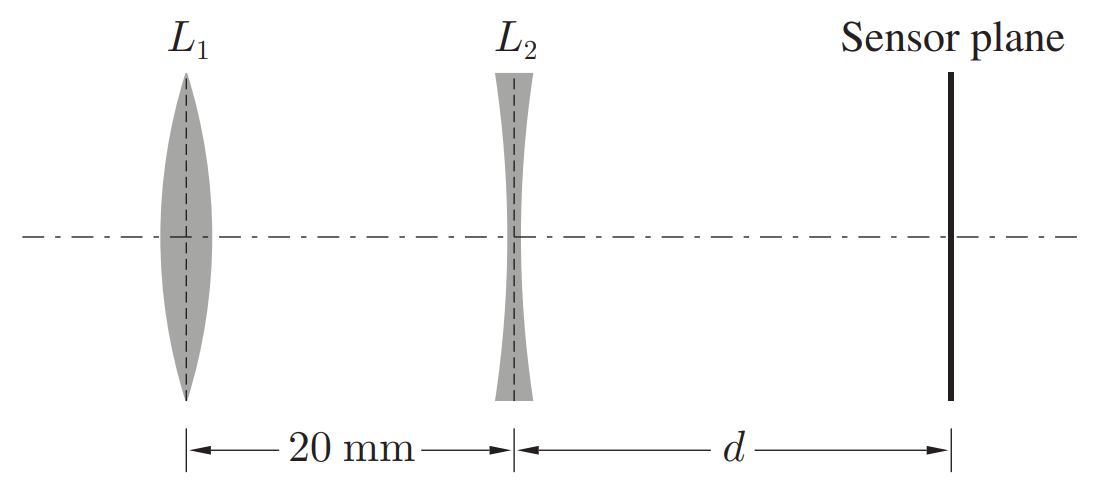
\includegraphics[width=0.35\linewidth]{Imágenes/clases/sensor.png}
\end{figure}

\end{enumerate}
\end{document}


% Para imágenes vectoriales -> el texto tiene que estar en LaTeX
% \begin{figure}[htbp]
%   \centering
%   \svgpath{../Imagenes/ejercicios}  -> .. irse pa'trás 
%   \includesvg{ej5.svg}
% \end{figure}
